\begin{figure*}[t]
    \centering
    
\includegraphics[width=0.98\linewidth]{figs/obsWM.pdf}
    \caption{
    Design space of observation-space world models. 
    The vertical axis denotes the spatial explicitness of the observation, ranging from RGB images to multi-view RGB, RGB-D, and point clouds. 
    The horizontal axis denotes the abstraction level of the action conditioning, ranging from low-level robot actions to interface actions, latent actions, and language instructions. 
    Different choices along these two axes lead to different trade-offs between spatial understanding, data availability, and downstream usability.
    }
    \label{fig:obs_space_wm}
\end{figure*}

\section{A Design-Space View of World Models}
\label{sec:design}

While Sec.~\ref{sec:definition} defines a world model abstractly as an action-conditioned predictive model, existing world models can be broadly categorized according to the space in which prediction is performed. 
As shown in Fig.~\ref{fig:overview}, we distinguish between two formulations: \emph{observation-space world models} and \emph{state-space world models}. 
An observation-space world model directly predicts future observations from past observations and actions. 
In contrast, a state-space world model first encodes observations into an internal state representation, and then predicts the future evolution in that state space. 
This distinction provides a useful starting point for organizing different world-modeling approaches, since it determines both what the model predicts and how the dynamics are represented.

\subsection{Observation-space World Models}
An observation-space world model predicts future observations directly in the observation space under a given action. 
Given an observation history $o_{0:t}$ and an action $a_t$, the model estimates the predictive distribution of the next observation:
\[
    o_{t+1} \sim p_\theta(\cdot \mid o_{0:t}, a_t),
\]
where $p_\theta$ is typically parameterized by a neural network. 
Under this formulation, the design space of observation-space world models can be largely characterized by two axes: the type of observation being predicted and the level of abstraction of the action conditioning, as illustrated in Fig.~\ref{fig:obs_space_wm}.

On the observation side, RGB images are the most common representation because they are easy to collect, require inexpensive and widely available sensors, and are abundant in Internet-scale video data ~\cite{gpc,dreamdojo,genie3,lingbot-world,rtfm,adaworld,cosmos,unipi,avdc,susie,v2a}. 
However, downstream decision-making tasks, especially robotic manipulation, often require the model to capture the spatial structure of the physical scene. 
This motivates the use of observations with increasing spatial explicitness, including multi-view RGB images ~\cite{ctrl-world,enerverse,vidar}, RGB-D images ~\cite{flowdreamer,roboscape,tesseract,clover, gvftape}, and point clouds ~\cite{particleformer,pointworld}. 
These representations provide progressively richer geometric information, but they also introduce a trade-off: spatially explicit data are much less available at scale than ordinary RGB videos. 
A common compromise is therefore to exploit large-scale RGB video data while enhancing their spatial information through monocular vision models, for example by annotating videos with estimated depth to form pseudo-RGB-D data ~\cite{flowdreamer, roboscape, tesseract, gvftape}.

On the action side, the choice of action representation is closely tied to the intended role of the world model. 
While the observation type determines what form of future is predicted, the action type largely determines how the model can be used. 
A more concrete action representation usually makes the model suitable for control and simulation, whereas a more abstract action representation often shifts the model toward pretraining, or planning.

At the most concrete level, actions correspond to low-level robot or agent commands, such as joint commands, end-effector actions, or continuous control signals ~\cite{particleformer, pointworld, flowdreamer, roboscape, ctrl-world, gpc, dreamdojo}. 
Since these actions are directly grounded in the embodiment of the agent, the resulting world model can predict the physical consequence of executing a specific control command. 
Such models are therefore commonly used as learned simulators for model-predictive control ~\cite{pointworld, particleformer,flowdreamer,gpc}, policy evaluation ~\cite{ctrl-world, roboscape}, or synthetic data generation ~\cite{ctrl-world, roboscape}.

At the next level, interface actions provide a controllable way to interact with the visual world without specifying the low-level motor commands of a particular embodiment. 
For example, given an initial image or scene context, the model may take user-level control signals, camera-control commands, or viewpoint-control inputs, and then synthesize the corresponding future observations ~\cite{genie3, lingbot-world, rtfm}. 
The purpose of this type of world model is not to predict robot dynamics, but to turn a static or partially observed scene into an interactive visual environment. 
It therefore serves as an interface-driven visual simulator, where users or agents can control how the scene is observed and obtain temporally consistent observations under different interactions.

Another line of work introduces latent actions, which are learned from unlabeled videos through reconstruction objectives with an information bottleneck~\cite{dreamdojo,adaworld}. 
Here, the action is not provided by the dataset, but inferred as a compact variable that explains the visual transition between frames. 
This design is mainly motivated by pretraining: by replacing missing action labels with learned latent actions, the world model can exploit large-scale action-free video data and acquire general dynamics priors before being adapted to downstream tasks.

At the most abstract level, actions can be represented as language instructions. 
Language-conditioned world models are less grounded in precise low-level control, but they are useful for high-level visual planning. 
Given a task description, such models generate possible future observations that describe how the task may unfold or be completed, thereby providing visual guidance for downstream agents ~\cite{tesseract, clover, enerverse, vidar, gvftape, cosmos, unipi, avdc, susie, v2a}.

\begin{figure*}[t]
    \centering
    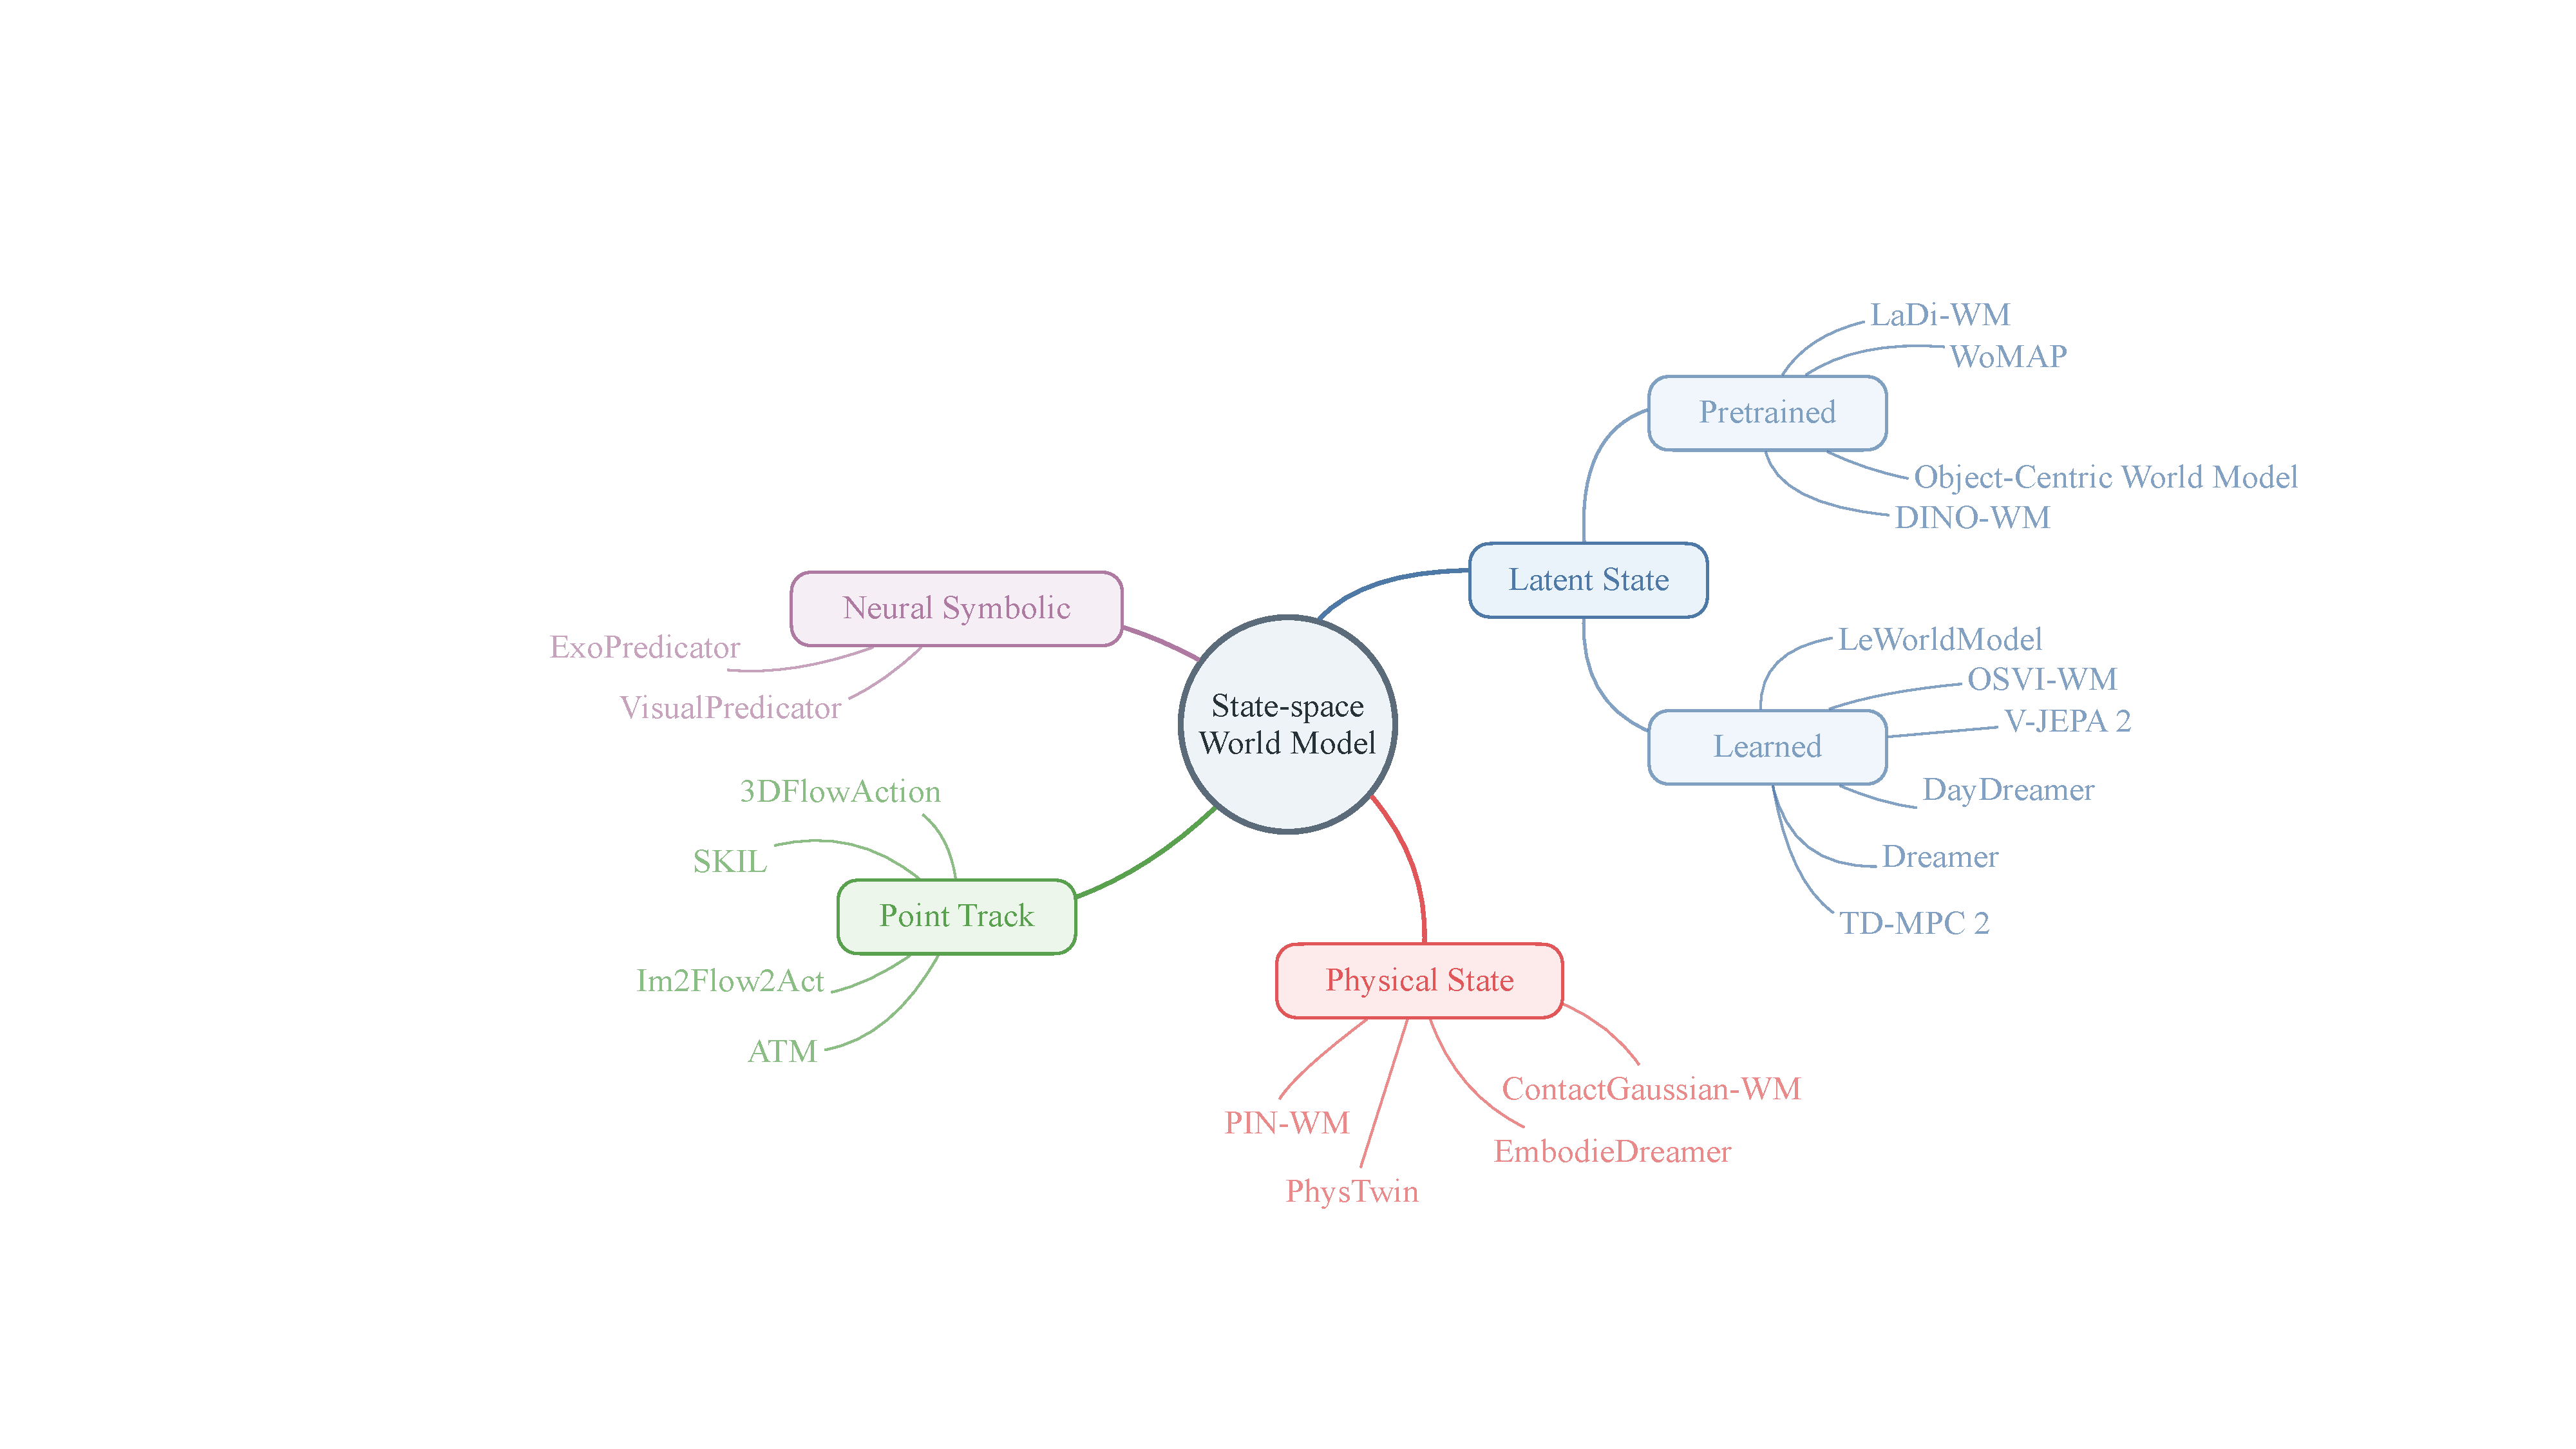
\includegraphics[width=0.98\linewidth]{figs/stateWM.pdf }
    \caption{
    Design space of state-space world models.
    Instead of predicting future observations directly in the raw observation space, state-space world models abstract observations into structured state representations and model their future evolution under actions.
    Representative state choices include latent states, point tracks, neural-symbolic predicates, and physical states.
    Different state representations provide different trade-offs between compactness, semantic structure, physical interpretability, scalability, and downstream usability.
    }
    \label{fig:state_space_wm}
\end{figure*}

\subsection{State-space World Models.}

Predicting future observations directly in the observation space is a natural formulation, but it is often difficult to learn because raw observations are high-dimensional and contain many task-irrelevant variations, such as background changes, illumination, texture, or sensor noise. As a result, modeling dynamics directly in the observation space may force the model to explain unnecessary visual details rather than the task-relevant evolution of the world. State-space world models address this issue by first abstracting observations into a more compact and structured state representation, and then predicting the future evolution in this state space:
\[
x_{t+1} \sim p(\cdot \mid o_{0:t}, a_t),
\]
where $x_{t+1}$ denotes the future state of interest, which may be a latent vector, a set of tracked points, a collection of symbolic predicates, or physical state variables. Different from observation-space world models, the transition model $p$ is not necessarily restricted to a neural network. Depending on the choice of state representation, the transition model may be implemented as a neural network, a symbolic or neural-symbolic operator model, or a physics-based simulator. By predicting structured states instead of raw observations, state-space world models reduce the complexity of dynamics learning and focus the prediction on task-relevant or physically meaningful aspects of the world. As illustrated in Fig.~\ref{fig:state_space_wm}, existing state-space world models can be organized according to the type of state representation they use.

A major class of state-space world models uses latent states, where observations are encoded into latent vectors by neural networks ~\cite{huang2025ladiwm,yin2025womap,jeong2025ocwm,zhou2024dinowm,maes2025leworldmodel,goswami2025osviwm,assran2025vjepa2,wu2022daydreamer,hafner2023dreamerv3,hansen2024tdmpc2}. These latent states can be obtained in different ways. Some methods learn the latent representation directly from the target domain, for example through reconstruction-based objectives ~\cite{wu2022daydreamer,hafner2023dreamerv3} or through predictive objectives that model future latent states without reconstructing pixels ~\cite{goswami2025osviwm,maes2025leworldmodel,assran2025vjepa2,hansen2024tdmpc2}. Such representations are usually adapted to the specific environment, task distribution, and control setting. Other methods use pretrained visual or vision-language models to extract latent features as state representations ~\cite{huang2025ladiwm,yin2025womap,jeong2025ocwm,zhou2024dinowm}. Since these encoders are trained on large-scale Internet data, the resulting states often provide more general semantic and visual abstractions. Latent-state world models are commonly paired with robot or agent actions, and are often used as compact learned simulators for reinforcement learning, or model-predictive control.

Another line of work represents the state as point tracks ~\cite{zhi20253dflowaction, wang2025skil, xu2024im2flow2act, wen2024atm}. These points can be two-dimensional ~\cite{wang2025skil, xu2024im2flow2act, wen2024atm} or three-dimensional ~\cite{zhi20253dflowaction}, randomly sampled ~\cite{wen2024atm} or semantically selected ~\cite{xu2024im2flow2act, zhi20253dflowaction, wang2025skil}, and their trajectories describe how task-relevant parts of the scene move over time. Compared with raw image prediction, point-track prediction removes much of the irrelevant background variation while preserving explicit motion information in the scene. This makes the future representation more compact and structured, without requiring the model to generate full visual observations. However, the choice of points also introduces an additional structural prior: although this prior can simplify learning, it may reduce scalability when the relevant scene elements are hard to define or vary significantly across tasks. In many applications, point-track world models are conditioned on language instructions and predict how key points in the scene should move in order to accomplish the task. The predicted tracks can then be used as reference trajectories or intermediate goals for a downstream controller.

Neural-symbolic world models use a set of grounded predicates as the state representation ~\cite{liang2025exopredicator, liang2024visualpredicator}. A neural-symbolic predicate is a symbolic Boolean fact whose truth value is grounded in raw perception by a neural model. This representation maps continuous visual observations into a compact set of logical facts that can support reasoning and planning. In this setting, actions are usually high-level skills rather than low-level motor commands. The transition model describes the preconditions and effects of these skills over the predicate state, similar in spirit to symbolic planning models such as PDDL, but with predicates grounded in perception. The goal of this type of world model is to learn a compact symbolic abstraction for long-horizon planning. By representing skills through their preconditions and effects, neural-symbolic world models support compositional reasoning, efficient search, and interpretable planning over high-level task structures.

A further class of state-space world models is based on physical states and classical mechanics ~\cite{li2025pinwm,jiang2025phystwin,wang2025embodiedreamer,wang2025contactgaussianwm}. Instead of learning arbitrary latent dynamics from data, these methods explicitly represent the world using physical variables such as object poses, velocities, contact states, masses, friction coefficients, or other dynamics parameters. This formulation incorporates strong human priors about how the physical world evolves, and is closely related to the modeling assumptions used in physics simulators. A typical pipeline first reconstructs the target scene in 3D, then aligns a simulated environment with the real scene by replaying real interaction trajectories and optimizing dynamics and rendering parameters. Once the simulator is aligned, future states can be predicted by solving physics-based transition equations conditioned on the current physical state and the agent action. Such world models are especially useful for model-predictive control, reinforcement learning, and synthetic data generation, where accurate physical rollouts are more important than directly generating raw visual observations.


